\documentclass[12pt,a4paper]{article}

\usepackage{a4wide}
\usepackage{fancyhdr}
\usepackage{graphicx}
\usepackage{epsfig}
\usepackage{parskip}
\usepackage[ansinew]{inputenc}
\usepackage{amsmath}
\usepackage{amssymb}
\usepackage{bm}
\usepackage{gensymb}
\usepackage[free-standing-units=true]{siunitx} % for consistent handling of SI units
\usepackage[colorlinks=true, pdfstartview=FitV, linkcolor=blue, citecolor=blue, urlcolor=blue]{hyperref} % enable links

\setlength{\parindent}{0pt}

\newcommand{\m}[1]
{\mathrm{#1}}

\title{Summary Experiment 09: "Absolute Zero"}
\author{Cedric Renda, Fritz Kurz}
\date{\today }

\begin{document}
	\maketitle

	\paragraph{Summary}
		In this experiment the goal is to determine the value of the absolute zero temperature. With $p$ as pressure, $V$ as Volume, $\nu$ as the amount of gas, R as a constant, T as temperature, the universal gas equation
		
			\begin{align}
				pV = \nu RT
			\end{align}
	
		 suggests that there is a linear correspondence between the pressure of a given amount of gas in a fix volume and the temperature. If we measure the pressure of this given amount and volume of gas at two known temperatures, we are able to calculate the absolute zero of temperature. 
		 
		 Because we can easily determine the temperature of the vapor of boiling water $t_k$ and ice $t_e$, we have the two needed temperatures to do the experiment. We first need to calibrate our pressure sensor, then fill a glass bulb with helium gas and measure the pressures $p_k$ and $p_e$ in the bulb at our two temperatures $t_k$ and $t_e$. We can then approximate the absolute zero of temperature $t_0$ with the following formula:
		 	
		 	\begin{align}
		 		t_0 \approx t_{00} = -\frac{p_e}{p_k - p_e}t_k
		 	\end{align}
	 	
		Here we did not take account of the errors in the experiment, so we have to use a more sophisticated calculation in the report. 
		
		After we calculate absolute zero, the bulb filled with gas works as a gas thermometer. In the second part of the experiment we want to measure the temperature of liquid nitrogen $t_N$. To do that, we submerge the bulb in the liquid and measure the pressure inside the bulb. We can then calculate the temperature of liquid nitrogen from that. 
		
		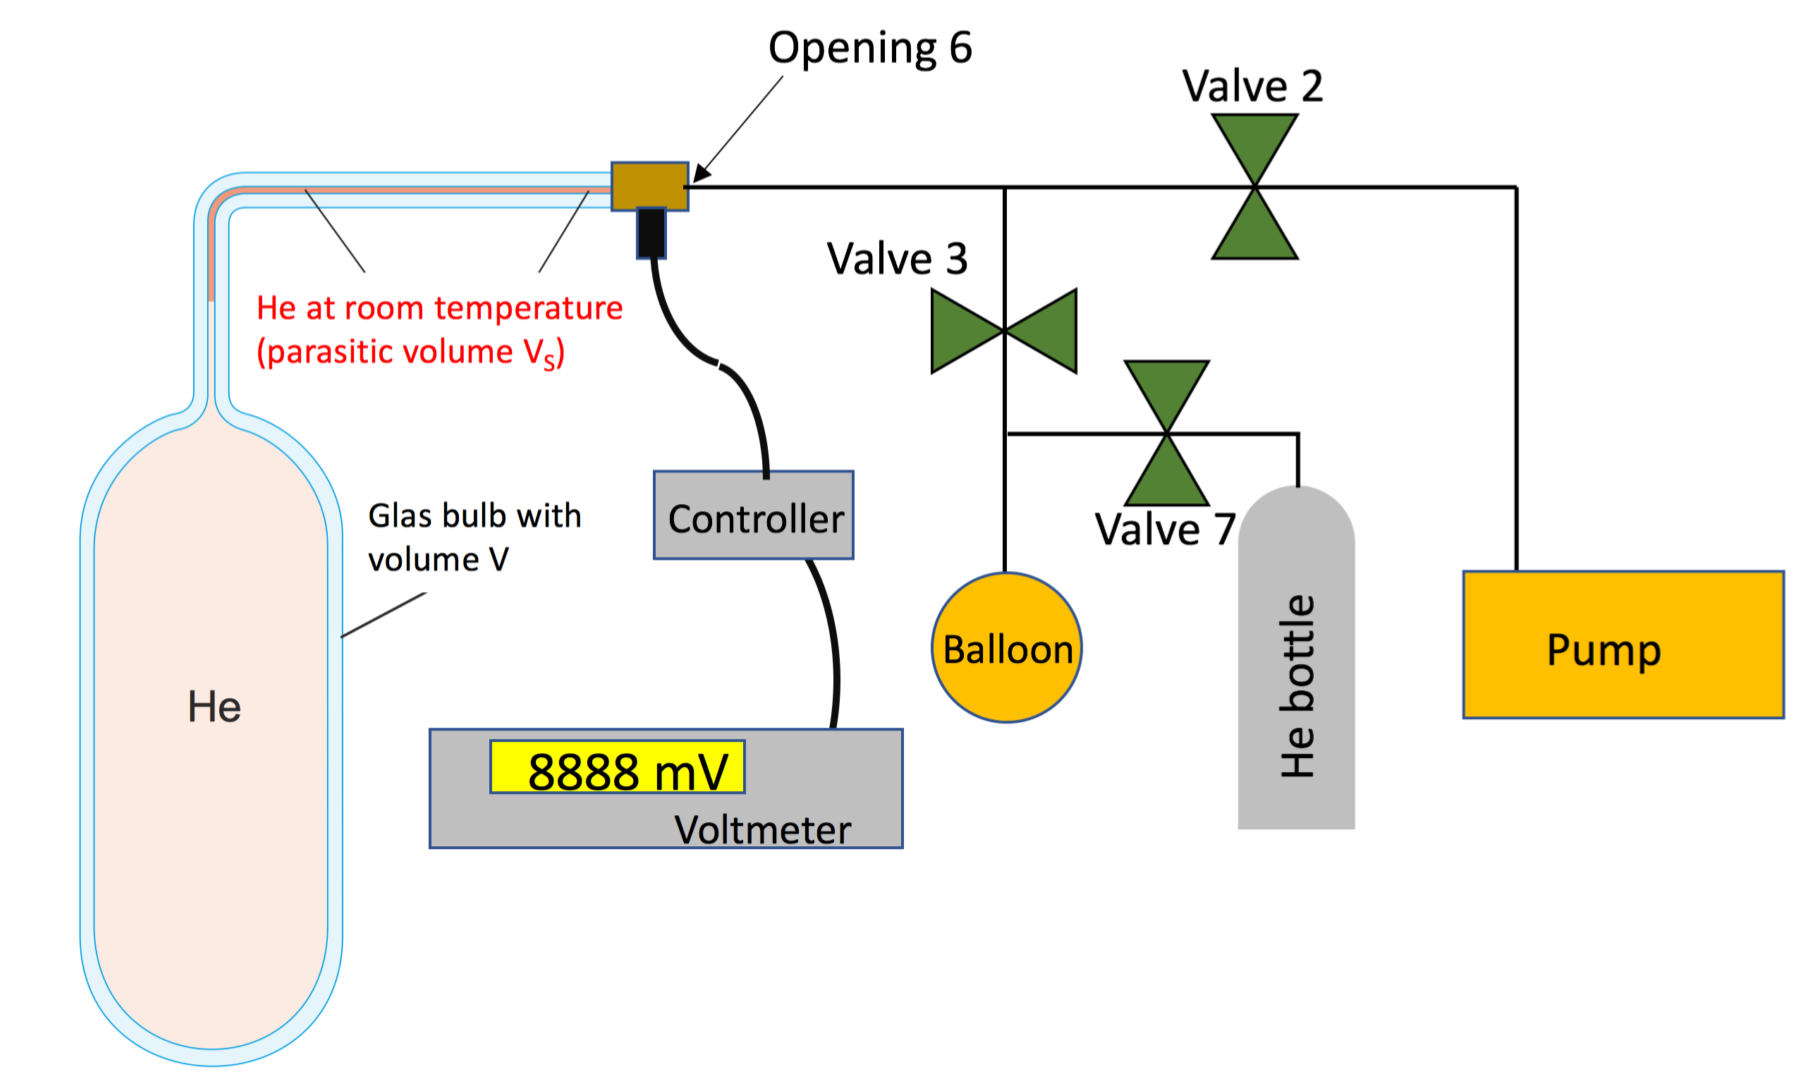
\includegraphics[width=\textwidth]{schematic.png}
\end{document}